\section{Analisi dinamica}
\note{Spostiamoci ora sulla parte dinamica}

\begin{frame}{Cosa è stato realizzato}
Si va a creare un sistema di sandbox, basato su Cuckoo Sandbox,
che esegue \emph{behavioural analysis} sul potenziale malware,
composto da una serie di VM
\begin{figure}
    \centering
    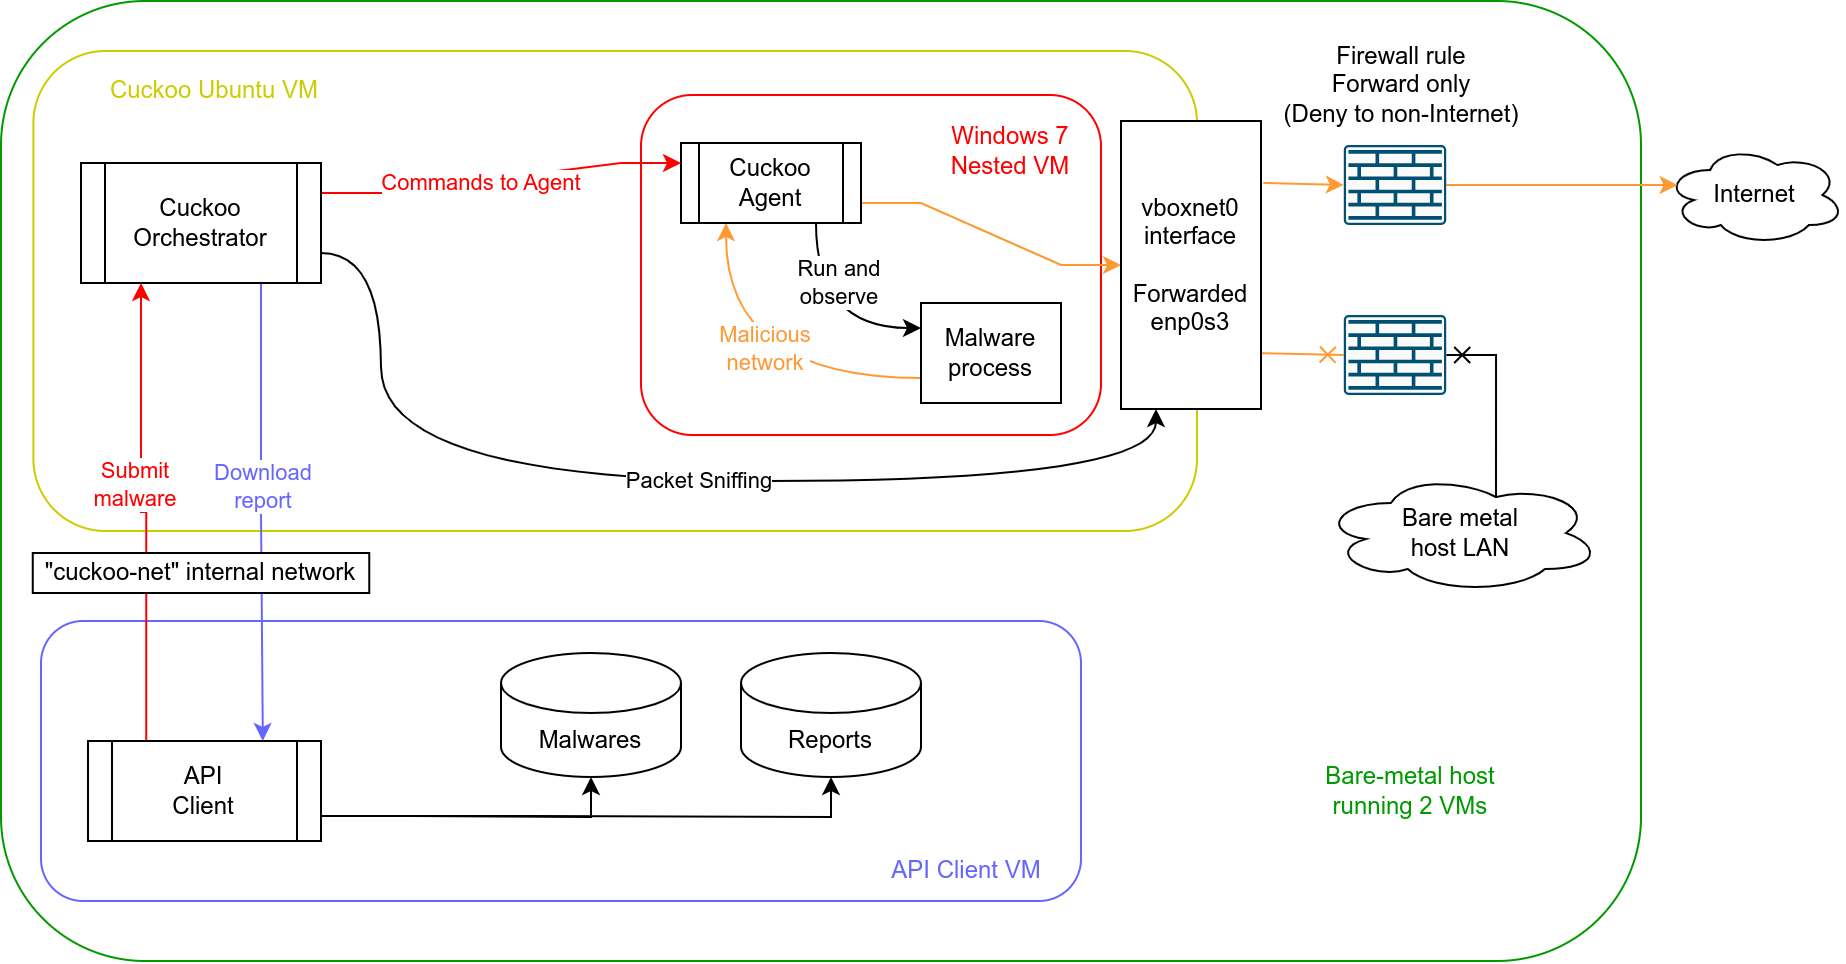
\includegraphics[width=0.75\textwidth]{images/cuckoo_vms.png}
\end{figure}

\note{
Si compone di:
\begin{itemize}
    \item una serie di macchine virtuali Virtualbox, anche innestate,
    \item poi configurate per massimizzare la sicurezza e l'isolamento,
    \item infine estese con altri plugin Python
\end{itemize}
%
La lunga configurazione del sistema ha previsto anche realizzazione di systemd unit, uso di Docker Compose per le dipendenze su servizi terzi (es: database) e uso di Virtualenv per poter usare Python 2 su VM Ubuntu.
}
\end{frame}

\begin{frame}{Anti VM-detection (1)}
\note{
Per rendere l'ambiente più verosimile possibile:
\begin{itemize}
    \item installiamo tutti programmi normalmente presenti, come browser, suite Office, PDF reader, WinRAR, ...
    \item allocando risorse di sistema reali, quali 4GB di RAM e 128GB di disco rigido
    \item installazione di runtime: service pack 1, Visual C++ redistributable, ...
\end{itemize}
%
Un malware potrebbe vedere l'assenza di un software sempre presente (es: Chrome) e decidere di non eseguire il reale comportamento malevolo, sospettando di essere analizzato
}

Si rende il sistema \textbf{verosimile}, installando programmi di utilità o molto diffusi, runtime, risorse come un computer scarso ma reale.
\vfill

\textbf{E tecniche più sofisticate} \\
Quali mitigazioni con DLL injection, uso di agent con OCR per simulare l'interazione umana, ...

\vfill
Superiamo \emph{quasi} ogni test di pafish (strumento per testare la VM detectability)
\end{frame}

% \begin{frame}{Anti VM-detection (2)}
% Si usa \textbf{pafish} come tool per capire quanto un malware possa rilevare di essere in un ambiente di analisi, con tecniche molto più sofisticate.

% Dopo uso di mitigazioni (DLL injection, agent con OCR, ...) quasi ogni test è superato:
% \begin{figure}
%   \centering
%   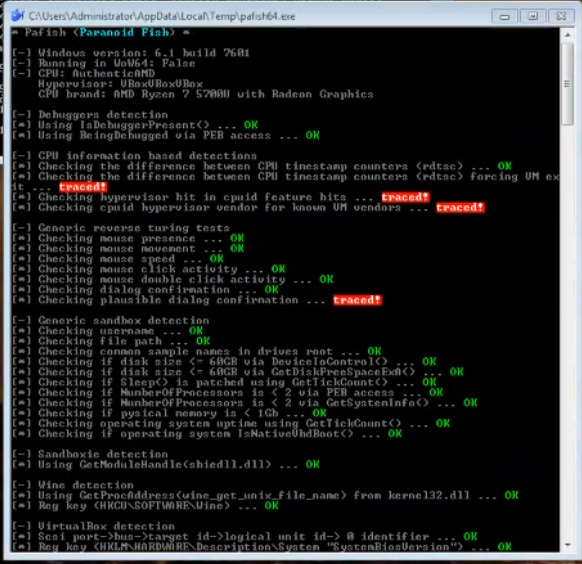
\includegraphics[width=0.4\textwidth]{images/pafish_cuckoo_1.png}
%   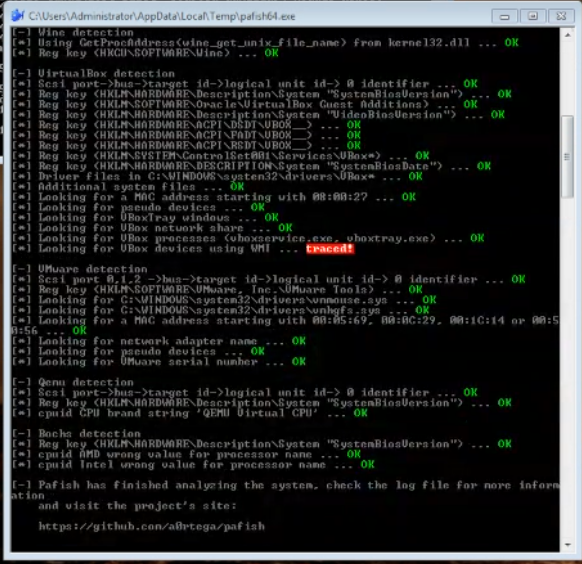
\includegraphics[width=0.4\textwidth]{images/pafish_cuckoo_2.png}
% \end{figure}
% \end{frame}

% \begin{frame}{Formato del report}
% Il report finale viene trasformato da ciò che fornirà Cuckoo di default.

% Vengono:
% \begin{itemize}
%     \item divise le syscall per thread, e non per processo
%     \item rimosse informazioni duplicate o poco chiare, organizzandole al meglio
%     \item ristrutturate le informazioni sul traffico di rete, dividendole per protocollo o categoria
% \end{itemize}
% \vfill
% Inoltre sono presenti screenshot, file creati dal malware e file PCAP della cattura dei pacchetti di rete
% \end{frame}

% \begin{frame}{Plugin (1)}
% Sono stati aggiunti nell'analisi anche due altri tool, ponendo le basi per come integrarne di diversi in futuro. Si compongono di più parti:
% \begin{itemize}
%     \item moduli \textbf{Auxiliary} e \textbf{Processing}, scritti in Python 2 usando le API di Cuckoo, eseguono rispettivamente nella VM Windows e nell'host Cuckoo per eseguire codice nelle due macchine, analizzare i risultati e interagire tra loro
%     \item server \textbf{HTTP} sull'host Cuckoo per rendere disponibile lo strumento al download da parte della VM sandbox
% \end{itemize}
% \end{frame}

\begin{frame}{Plugin} % {Plugin (2)}
\note{è stata estesa la potenza della sandbox sviluppando dei plugin in Python per aggiungere altri tool, di per sè non supportati.}
I tool integrati sono:
\begin{itemize}
    \item \textbf{Patriot}, che rileva tecniche \emph{in-memory stealth}
    \item \textbf{Hunt-Sleeping-Beacons} per tattiche particolari di sleep obfuscation
\end{itemize}
\note{
\begin{itemize}
    \item \textbf{Patriot}, rileva tecniche di occultamento in memoria (\emph{in-memory stealth}), usate anche da Cobalt Strike
    \item \textbf{Hunt-Sleeping-Beacons}, identifica processi che stanno in stato di Sleep ma in modi non standard e non rilevabili tradizionalmente, come \emph{Foliage}; quindi contro sleep obfuscation
\end{itemize}
.
}
\Pause

\vfill
\note{Questo apre anche le porte a una futura integrazioni di strumenti sempre più recenti, basterà creare un plugin seguendo questo stesso schema. \textbf{COMPONENTI SLIDE}}
Integrati con più componenti:
\begin{itemize}
    \item Modulo \textbf{auxiliary} per eseguire nella VM
    \item Modulo \textbf{processing} per analizzare gli output raw
    \item Server \textbf{HTTP} per scaricare il tool prima dell'analisi
\end{itemize}
\end{frame}

\begin{frame}{Hardening}
Si adottano tecniche per fare l'hardening della sandbox:
\note{
\begin{itemize}
    \item a livello di \textbf{rete} viene usato un firewall per impedire che la sandbox possa contattare altri dispositivi nella rete dell'host, servizi dell'agent che non dovrebbero essere esposti, e forwarding dei pacchetti dalla sandbox all'interfaccia di rete sotto sniffing indirizzati verso Internet
    \\\hrulefill
    \item a livello di \textbf{utente} viene creato uno Unix user senza login shell e con i minimi privilegi per ridurre la superficie di attacco se compromessa la VM dove esegue Cuckoo
    \\\hrulefill
    \item ripristino \textbf{snapshot} della VM Windows dopo ogni analisi per ripristinare sempre lo stato pulito e iniziale
    \\\hrulefill
    \item creazione di un'\textbf{altra VM} su rete interna (non connessa a Internet) per interagire con la VM sandbox e salvare sample e risultati
\end{itemize}
}
\begin{itemize}
    \item Firewall, per proteggere a livello di \textbf{rete}
    \pause
    \item Utente Linux separato per eseguire Cuckoo
    \pause
    \item ripristino \textbf{snapshot} dopo ogni analisi
    \pause
    \item creazione di un'\textbf{altra VM} su rete interna
\end{itemize}
\end{frame}

% \begin{frame}{Client Python}
% Per interagire con la sandbox, si è creato un client Python.

% \begin{enumerate}
%     \item Astrae l'uso della REST API di Cuckoo tramite delle apposite classi (può essere riciclato il codice in futuro)
%     \item Fornisce un'interfaccia utente all'analista più semplice di una web UI (che è stata limitata in fase di Hardening)
% \end{enumerate}
% \end{frame}

% \begin{frame}{Architettura finale}
% \begin{figure}
%     \centering
%     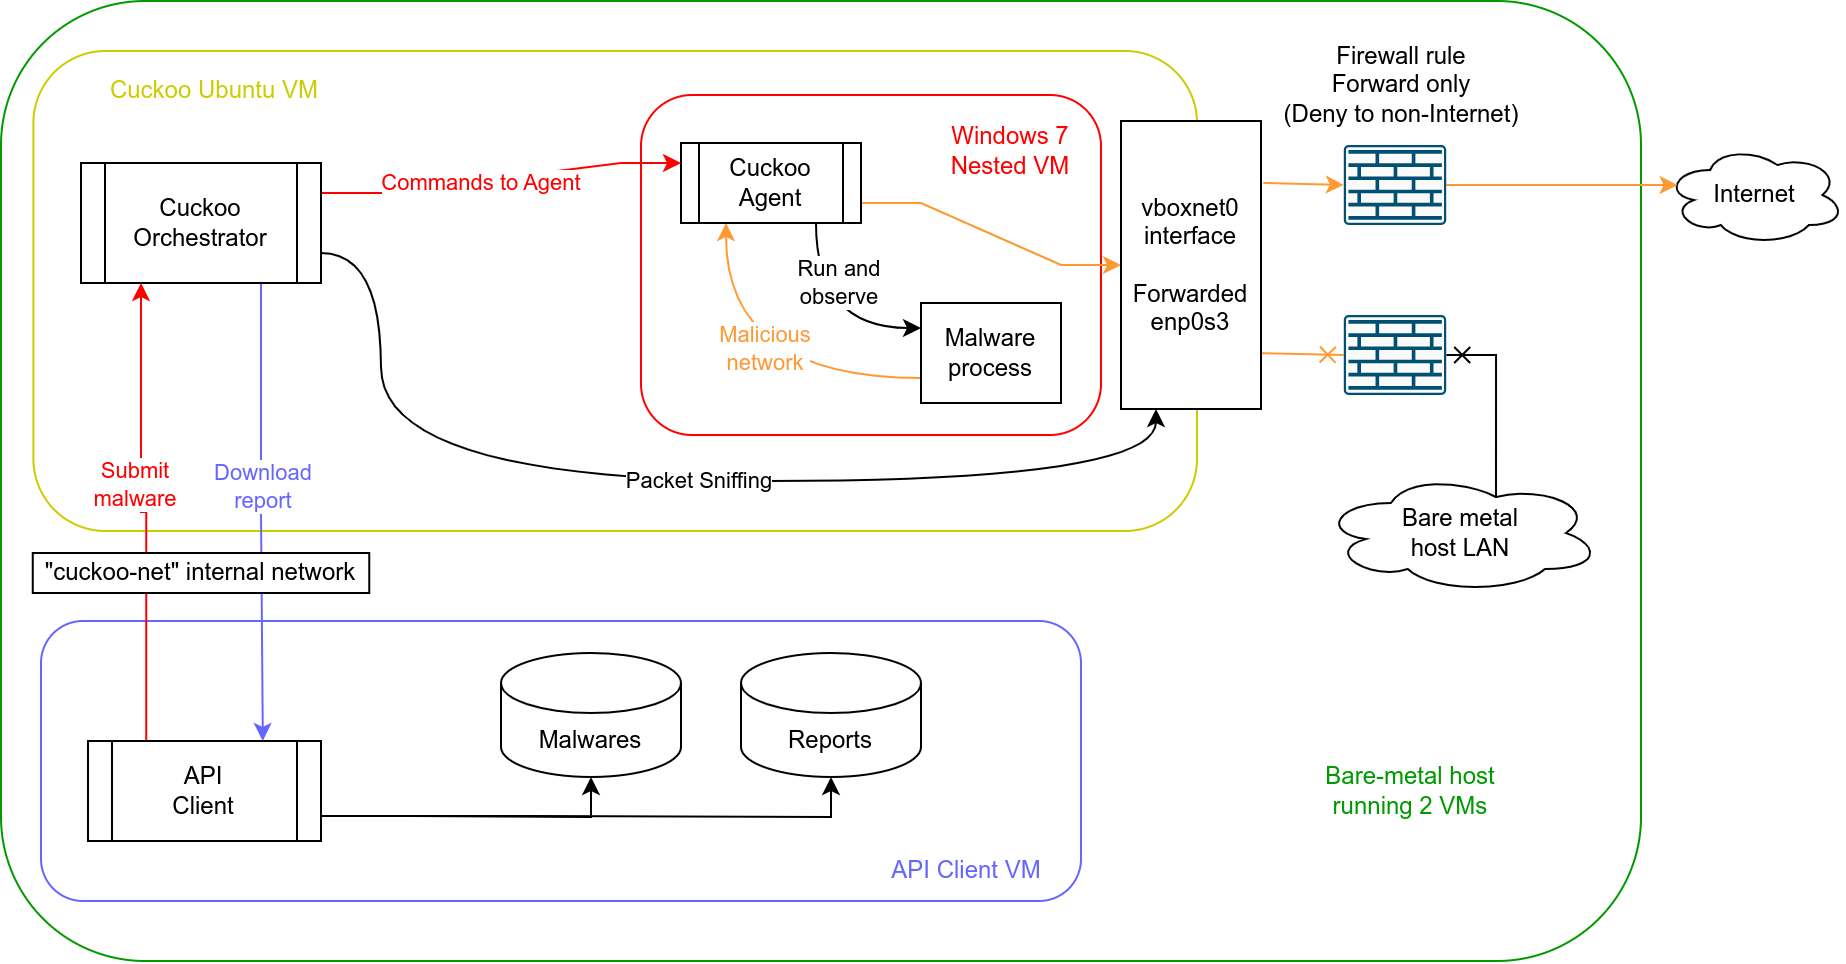
\includegraphics[width=0.9\textwidth]{images/cuckoo_vms.png}
% \end{figure}
% \end{frame}

\begin{frame}{Client Python per l'interazione}
\begin{figure}
    \centering
    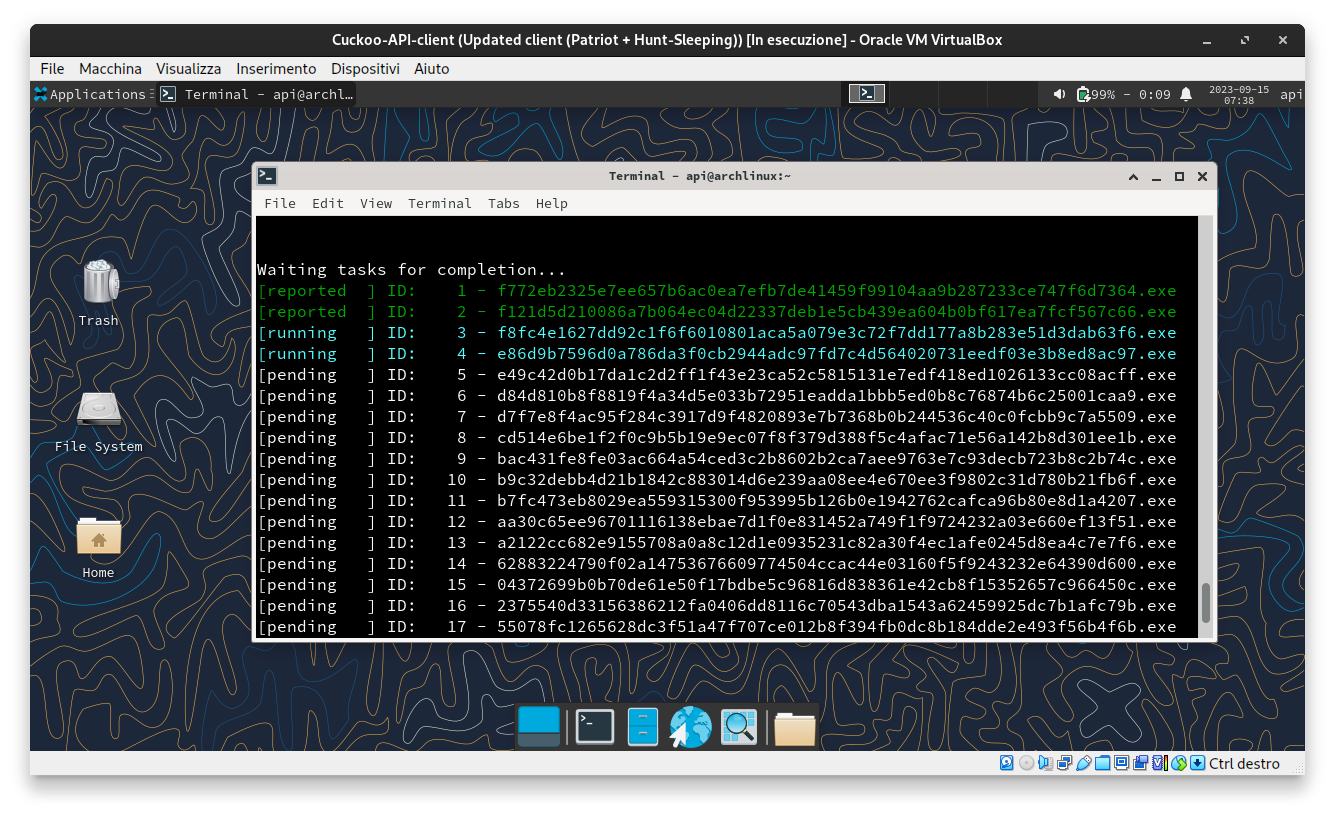
\includegraphics[width=0.8\textwidth]{images/dynamic-api-client-running.png}
\end{figure}
\note{
Per interagire con la sandbox, si è creato un client Python.
Qui vediamo lo screenshot della sua esecuzione in modalità interattiva.
\\
\begin{enumerate}
    \item Astrae l'uso della REST API di Cuckoo tramite delle apposite classi (può essere riciclato il codice in futuro, riducendo il rischio di introdurre bug derivanti da una nuova implementazione)
    \item Fornisce un'interfaccia utente all'analista più semplice di una web UI (che è stata limitata in fase di Hardening)
\end{enumerate}
}
\end{frame}

\begin{frame}{Interfaccia dalla VM Client (2)}
\begin{figure}
    \centering
    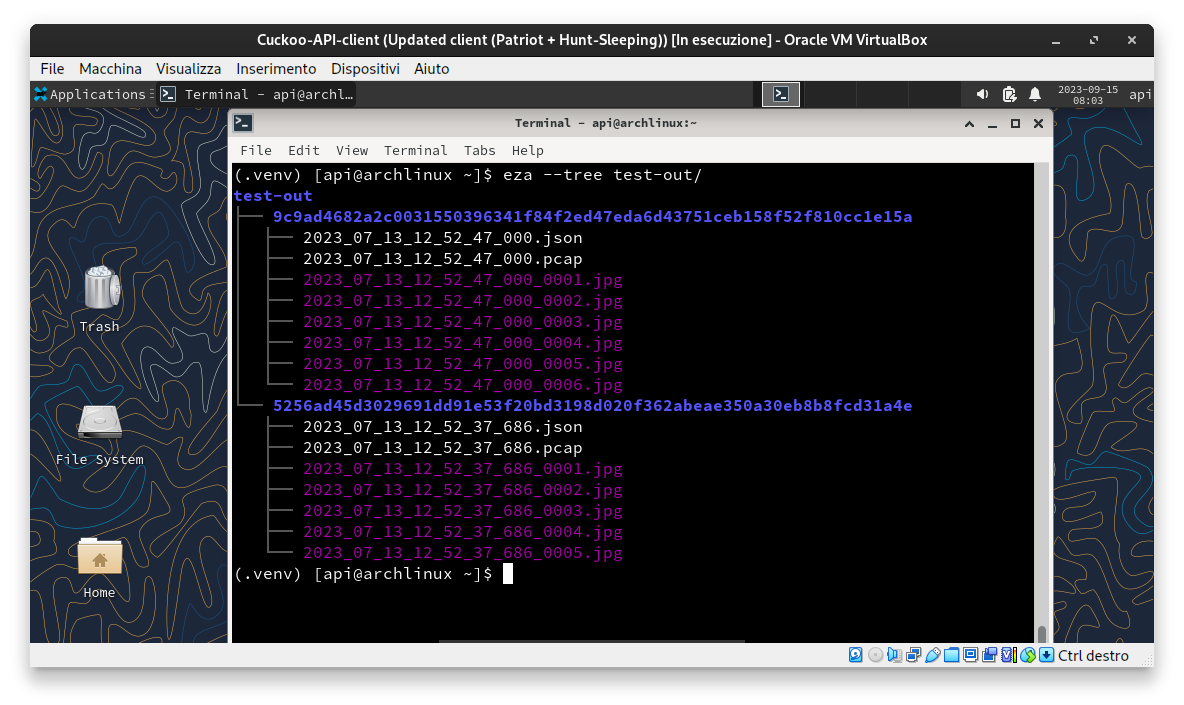
\includegraphics[width=0.8\textwidth]{images/dynamic-api-results.png}
\end{figure}
\note{
Il report finale viene trasformato da ciò che fornirà Cuckoo di default.
%
Vengono:
\begin{itemize}
    \item divise le syscall per thread, e non per processo
    \item rimosse informazioni duplicate o poco chiare, organizzandole al meglio
    \item ristrutturate le informazioni sul traffico di rete, dividendole per protocollo o categoria
\end{itemize}
%
Inoltre sono presenti screenshot, file creati dal malware e file PCAP della cattura dei pacchetti di rete
}
\end{frame}